\documentclass[11pt]{article}
\usepackage[paper=a4paper,margin=2cm]{geometry}
\usepackage[svgnames]{xcolor}
\usepackage{listings}
\usepackage{sourcecodepro}
\usepackage{graphicx}

\graphicspath{ {./images/} }

\lstset{
    language=R,
    basicstyle=\footnotesize\ttfamily,
    stringstyle=\color{DarkGreen},
    commentstyle=\color{DarkBlue},
    keywordstyle=\footnotesize\ttfamily,
    showstringspaces=false,
    deletekeywords={/},
    xleftmargin=.35em,
    xrightmargin=.35em,
}

\begin{document}

\section*{Pergunta 1}

\begin{lstlisting}
    library(ggplot2)
    theme_set(theme_light())

    dados <- read.csv("./data/Paises_PIB_ICH.csv")
    continentes <- c("Asia", "Africa")
    paises <- c("United Arab Emirates", "Nepal", "Comoros", "Namibia")

    dados <- dados[dados$Continent %in% continentes,]

    ggplot(dados, aes(x = GDP, y = HCI)) +
        geom_point(size = 3, aes(color = Continent, shape = Continent)) +
        scale_shape_manual(values = c(16, 18)) +
        scale_x_log10() +
        geom_text(data = subset(dados, Country %in% paises), aes(label = Country), 
                  vjust = -1, hjust = 0.5, size = 3.5) +
        labs(title = "Human Capital Index relative to GDP per capita",
             subtitle = "In Asian and African countries",
             x = "GDP per capita [2023]",
             y = "Human Capital Index [2020]")
\end{lstlisting}

\vspace{14pt}

\begin{center}
    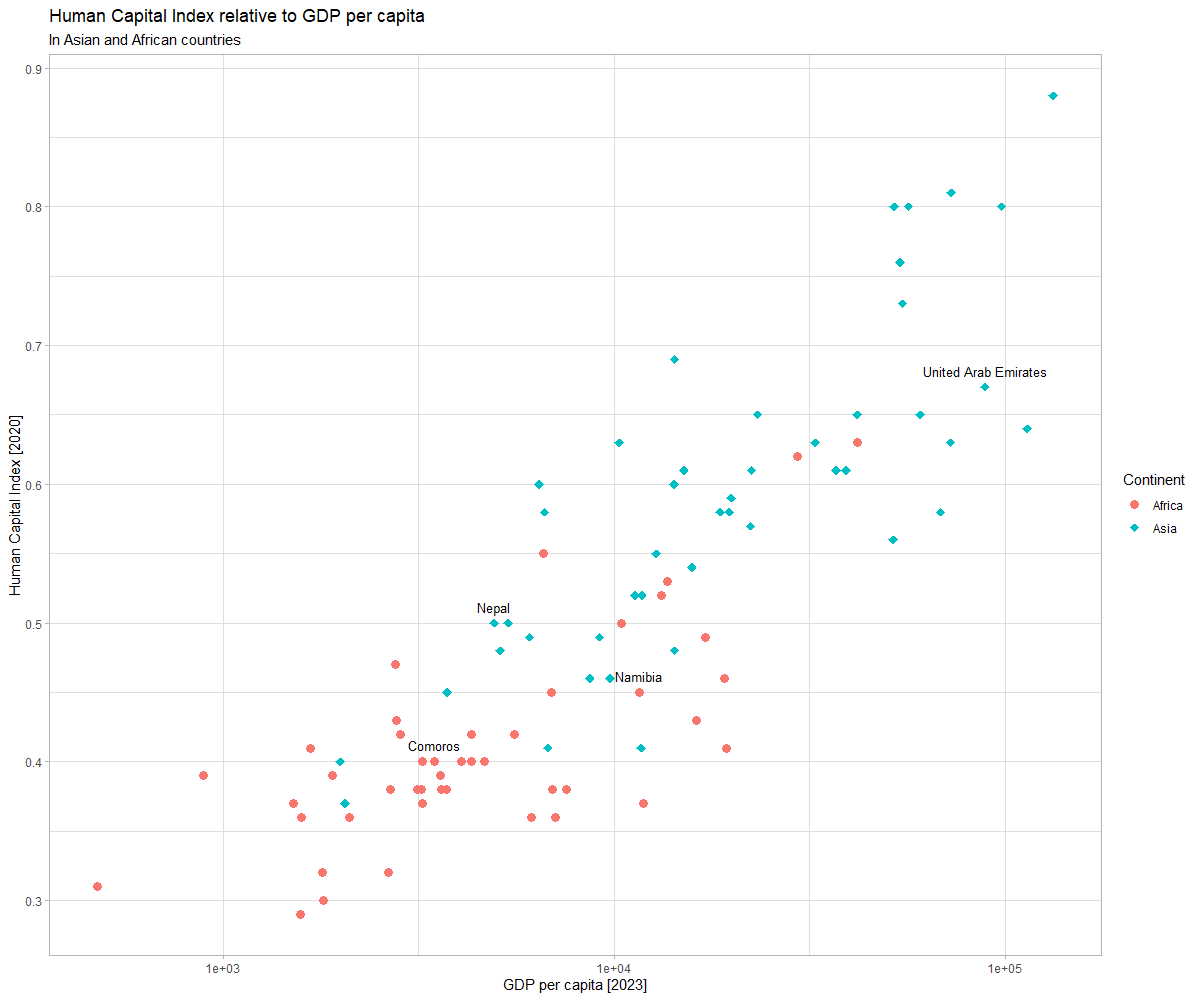
\includegraphics[width=\linewidth]{pergunta_1.png}
\end{center}

\end{document}